% Informe del Proyecto 1 (Entregable 1) — MiniDB
% Compilar:  cd docs/informe && tectonic informe.tex      (o latexmk -pdf informe.tex, o Overleaf)
\documentclass[11pt,a4paper]{article}

\usepackage{iftex}
\ifPDFTeX
  \usepackage[utf8]{inputenc}
  \usepackage[T1]{fontenc}
  \usepackage{lmodern}
\else
  \usepackage{fontspec}
\fi
\usepackage[spanish,es-noshorthands,es-tabla,es-nodecimaldot]{babel}
\usepackage[margin=2.2cm]{geometry}
\usepackage{amsmath,amssymb}
\usepackage{graphicx}
\usepackage{booktabs}
\usepackage{tabularx}
\usepackage{array}
\usepackage{multirow}
\usepackage{xcolor}
\usepackage{listings}
\usepackage{caption}
\usepackage{subcaption}
\usepackage{float}
\usepackage{enumitem}
\usepackage{tikz}
\usetikzlibrary{positioning,arrows.meta,calc,fit}
\usepackage[hidelinks]{hyperref}

\graphicspath{{figuras/}}
\setlength{\parskip}{0.35em}
\setlist{itemsep=0.15em,topsep=0.3em}
\captionsetup{font=small,labelfont=bf}

\definecolor{codebg}{RGB}{246,248,250}
\definecolor{kw}{RGB}{0,92,197}
\lstdefinestyle{sql}{
  language=SQL, basicstyle=\ttfamily\small, keywordstyle=\color{kw}\bfseries,
  backgroundcolor=\color{codebg}, frame=single, rulecolor=\color{black!15},
  columns=fullflexible, breaklines=true, morekeywords={USING,HEAP,SEQUENTIAL,BTREE,HASH,COPY,EXPLAIN,BETWEEN,INDEX}
}
\lstdefinestyle{txt}{basicstyle=\ttfamily\small, backgroundcolor=\color{codebg}, frame=single,
  rulecolor=\color{black!15}, columns=fullflexible, breaklines=true}
\newcommand{\code}[1]{\texttt{#1}}

\title{\textbf{MiniDB: gestor de bases de datos relacional en disco}\\[0.3em]
\large Proyecto 1 (Entregable 1) --- Base de Datos II (CS2042) --- UTEC 2026-II\\
\normalsize Docente: Percy Lovon Ramos}
\author{Renzo Acervo \and Josué Toribio \and \emph{(integrante 3)} \and \emph{(integrante 4)}}
\date{Septiembre de 2026}

\begin{document}
\maketitle

\begin{abstract}
\noindent MiniDB es un gestor de bases de datos relacional construido desde cero en Python que opera
directamente sobre memoria secundaria. Todo dato e índice vive en archivos binarios organizados en
páginas de tamaño fijo que se transfieren de a una con \code{seek} + \code{read}/\code{write} y se
serializan con \code{struct}. Implementamos un Heap File con \emph{free-list}, un Sequential File
con área de overflow encadenada y reorganización con \emph{fill factor}, un árbol B$^+$ multinivel y
un Extendible Hashing, ambos en disco; un motor SQL propio (lexer, parser de descenso recursivo,
planificador con estimación de costos y ejecutor), una API REST y un cliente web de cuatro paneles.
Un monitor \code{DiskCounter} registra exactamente las páginas leídas y escritas por cada sentencia.
Con 100\,000--500\,000 registros sintéticos, los cuatro experimentos pedidos reproducen los costos
teóricos: la inserción en el Heap cuesta 2 I/O, la búsqueda puntual cuesta $P$ lecturas con full scan,
$\lceil\log_2 M\rceil$ con búsqueda binaria, $h+1$ con el B$^+$ y 3 con el hash, y un índice no agrupado
deja de convenir frente al full scan cuando el rango supera $\approx P/N$ de la tabla.
\end{abstract}

\tableofcontents
\newpage

%==========================================================================================
\section{Introducción}

El cuello de botella de un gestor de bases de datos es la transferencia de bloques entre disco y
memoria, por lo que el costo de cada operación se mide en páginas transferidas. El objetivo de este
entregable es construir el núcleo relacional de un gestor que haga visible ese costo: cada estructura
se diseña para minimizar el número de accesos a disco y cada consulta informa exactamente cuántos hizo.

\paragraph{Alcance.} El sistema implementa todos los componentes del Entregable 1:
almacenamiento paginado con \code{DiskCounter}; Heap File y Sequential File; árbol B$^+$ y hashing
dinámico en disco; SQL con \code{CREATE TABLE}, \code{INSERT}, \code{SELECT ... WHERE},
\code{DELETE} y \code{CREATE INDEX} (más \code{DROP}, \code{COPY} y \code{EXPLAIN}); planificador
con desglose de I/O y latencia; API REST; cliente web y experimentación con hasta 500\,000 registros.

\paragraph{Restricciones respetadas.} No se usa ningún motor de bases de datos ni ORM; ningún
archivo se serializa con \code{pickle}, \code{json} o similares (todo es \code{struct} little-endian);
nunca se lee un archivo completo: solo \code{f.seek(offset)} + \code{f.read(page\_size)}; no hay
\code{mmap} y todo acceso a disco pasa por \code{DiskManager}; la función hash persistida es
\code{zlib.crc32} (no \code{hash()}, que en Python está salteado por proceso); y ninguna operación
carga una tabla completa en memoria (ni siquiera \code{reorganize}, que usa ordenamiento externo si
hace falta).

\paragraph{Tecnologías.} Backend en Python~3.12 con FastAPI; frontend en React + TypeScript (Vite)
con CodeMirror~6 y Recharts; todo se levanta con \code{docker compose up --build}. Los benchmarks usan
matplotlib solo para graficar.

%==========================================================================================
\section{Arquitectura del sistema}

\begin{figure}[H]
\centering
\begin{tikzpicture}[
  box/.style={draw, rounded corners=2pt, minimum width=3.6cm, minimum height=0.75cm, align=center, font=\small, fill=white},
  wide/.style={box, minimum width=11.6cm},
  arr/.style={-{Stealth[length=2mm]}, thick}]
\node[wide, fill=blue!6] (web) {Cliente web (React): explorador $\cdot$ editor SQL $\cdot$ resultados $\cdot$ plan y métricas};
\node[wide, below=0.45cm of web, fill=blue!3] (api) {API REST (FastAPI) --- \code{Database}: catálogo, tablas abiertas, lock, \code{DiskCounter} por sentencia};
\node[box, below left=0.45cm and -3.6cm of api] (lex) {Lexer + Parser\\(descenso recursivo)};
\node[box, right=0.4cm of lex] (plan) {Planner\\(reglas + costos)};
\node[box, right=0.4cm of plan] (exec) {Executor\\(filtros, paginación)};
\node[box, below=0.9cm of lex, fill=orange!8] (heap) {HeapFile\\(free-list)};
\node[box, right=0.4cm of heap, fill=orange!8] (seq) {SequentialFile\\(+ overflow)};
\node[box, right=0.4cm of seq, fill=green!8] (idx) {BPlusTree $\cdot$ ExtendibleHash};
\node[wide, below=0.45cm of seq, fill=gray!10] (dm) {\code{DiskManager}: \code{seek(page\_id $\cdot$ B)} + \code{read/write(B)}; cuenta \code{disk\_reads} / \code{disk\_writes}};
\node[wide, below=0.45cm of dm, fill=gray!4] (disk) {Archivos binarios paginados: \code{catalog.bin}, \code{*.heap}, \code{*.seq}, \code{*.ovf}, \code{*.bpt}, \code{*.hsh}};
\draw[arr] (web) -- (api);
\draw[arr] (api.south) -- ++(0,-0.2) -| (lex.north);
\draw[arr] (lex) -- (plan);
\draw[arr] (plan) -- (exec);
\draw[arr] (exec.south) -- (idx.north);
\draw[arr] (exec.south) -- (seq.north);
\draw[arr] (exec.south) -- (heap.north);
\node[fit=(heap)(seq)(idx), inner sep=2pt] (tbl) {};
\draw[arr] (seq.south) -- (dm.north);
\draw[arr] (dm) -- (disk);
\end{tikzpicture}
\caption{Capas de MiniDB. Todo acceso a disco pasa por \code{DiskManager}, que cuenta cada página transferida.}
\label{fig:arquitectura}
\end{figure}

Una consulta sigue el camino de la figura~\ref{fig:arquitectura}: el cliente envía el SQL a
\code{POST /api/query}; \code{Database.execute} lo parsea sentencia por sentencia (el lexer produce
tokens de forma perezosa, así el tiempo de parseo de cada sentencia se mide por separado), resetea el
\code{DiskCounter} compartido, ejecuta la sentencia, persiste las páginas~0 que cambiaron y devuelve
filas paginadas, el plan y las métricas (\code{disk\_reads}, \code{disk\_writes}, \code{parse\_ms},
\code{exec\_ms}, \code{total\_ms}, medidos con \code{time.perf\_counter()}). Un \emph{lock} serializa
las sentencias: el motor atiende una a la vez, de modo que el conteo de cada una es exacto.

La clase \code{Table} agrupa el archivo de datos (Heap o Sequential) y sus índices, y mantiene la
consistencia entre ellos: todo \code{INSERT} y \code{DELETE} actualiza todos los índices y, tras una
reorganización del Sequential, los índices se reconstruyen porque los RID cambian.

%==========================================================================================
\section{Diseño físico}

\subsection{DiskManager y DiskCounter}

Cada archivo es un \code{DiskManager} que lo abre una sola vez en modo \code{r+b} y \textbf{sin buffer
de Python} (\code{buffering=0}): cada \code{read\_page(i)} es exactamente un \code{seek(i$\cdot$B)} y
un \code{read(B)}, y cada \code{write\_page} un \code{seek} y un \code{write} de la página completa
(se valida que \code{len(data) == B}). No hay \emph{buffer pool}: así el número de páginas
transferidas coincide con el costo teórico de cada algoritmo. \code{allocate\_page()} solo reserva
el siguiente \code{page\_id} (sin I/O); la escritura del contenido inicial es la que se cuenta, de
modo que agregar una página cuesta una escritura. El tamaño de página $B$ es un parámetro
\textbf{por archivo} (1024 a 8192 bytes en el Experimento~4, 4096 por defecto) y se guarda en la
página~0.

El \code{DiskCounter} tiene exactamente las dos variables pedidas, \code{disk\_reads} y
\code{disk\_writes}; se comparte entre todos los archivos de una ejecución y se resetea antes de cada
sentencia.

\subsection{Header común de página}

Todas las páginas de todos los archivos empiezan con el mismo header de 24 bytes, empaquetado como
\code{'<IBBHHiiixx'} (tabla~\ref{tab:header}).

\begin{table}[H]
\centering\small
\begin{tabular}{@{}lrrl>{\raggedright\arraybackslash}p{7.2cm}@{}}
\toprule
Campo & Offset & Bytes & Tipo & Uso \\
\midrule
\code{page\_id} & 0 & 4 & u32 & identificador del bloque dentro del archivo \\
\code{page\_type} & 4 & 1 & u8 & 0 META, 1 HEAP, 2 SEQ\_MAIN, 3 SEQ\_OVERFLOW, 4 B$^+$ interno, 5 B$^+$ hoja, 6 HASH\_DIR, 7 HASH\_BUCKET, 8 CATALOG, 9 SORT\_RUN \\
\code{flags} & 5 & 1 & u8 & específico del tipo (profundidad local del bucket) \\
\code{record\_count} & 6 & 2 & u16 & registros o claves activos en la página \\
\code{free\_space\_offset} & 8 & 2 & u16 & primer slot libre (\code{0xFFFF} = llena) o fin de los datos usados \\
\code{next\_page\_id} & 10 & 4 & i32 & encadenamiento (free-list, overflow, \code{next\_leaf}); $-1$ = nulo \\
\code{prev\_page\_id} & 14 & 4 & i32 & encadenamiento (\code{prev\_leaf}, página principal anterior) \\
\code{aux\_page\_id} & 18 & 4 & i32 & específico (cabeza del overflow de una página principal) \\
relleno & 22 & 2 & -- & alineación a 24 bytes \\
\bottomrule
\end{tabular}
\caption{Header de página (24 bytes, little-endian).}
\label{tab:header}
\end{table}

\paragraph{Página 0 de metadatos.} Tras el header, la página~0 de cada archivo guarda
\code{magic} (\code{MDB1}), versión, tipo de archivo, \code{page\_size} y \code{num\_pages}
(16 bytes) y luego los campos propios de cada estructura: cabeza de la free-list y número de registros
(Heap); capacidad, columna clave, fill factor y mínimo/máximo de la PK (Sequential); raíz, altura,
capacidades y número de hojas (B$^+$); profundidad global y la tabla de segmentos del directorio (hash).
La página~0 se lee una vez al abrir el archivo y queda en memoria. Al final de cada sentencia se
escribe \textbf{solo si cambió su estructura} (cabeza de la free-list, raíz o altura del B$^+$,
directorio del hash); las estadísticas (número de registros, mínimo y máximo de la clave) viajan en esa
escritura o al cerrar el archivo. Tanto la lectura al abrir como estas escrituras se cuentan en el
\code{DiskCounter}: por ejemplo, el \code{INSERT} que obliga a crear una página nueva del Heap cuesta
1W de la página nueva más 1W de la página~0 (cambió la cabeza de la free-list), mientras que un
\code{INSERT} en una página que ya tenía espacio cuesta exactamente 1R + 1W.

\subsection{Registros de longitud fija con bitmap y RID}

Elegimos registros de longitud fija con bitmap de presencia. Los tipos se empaquetan con
\code{struct}: \code{INT}$\to$\code{'i'} (4 B), \code{FLOAT}$\to$\code{'d'} (8 B) y
\code{CHAR(n)}/\code{VARCHAR(n)}$\to$\code{'ns'} (UTF-8 rellenado con \code{\textbackslash x00}; se
trunca por bytes sin cortar un carácter multibyte). La tabla del enunciado,
\code{empleados(id INT, nombre CHAR(30), dept CHAR(20), salario FLOAT)}, se empaqueta como
\code{'<i30s20sd'} = 62 bytes. Una página de datos tiene el layout
\[
\underbrace{\text{header}}_{24\ \text{B}}\;\big|\;\underbrace{\text{bitmap}}_{\lceil cap/8\rceil\ \text{B}}\;\big|\;\underbrace{\text{slot}_0 \cdots \text{slot}_{cap-1}}_{cap\,\times\,62\ \text{B}}
\qquad\text{con}\qquad cap=\max\{n : 24+\lceil n/8\rceil+62n \le B\}.
\]

\begin{table}[H]
\centering\small
\begin{tabular}{@{}lrrrr@{}}
\toprule
$B$ (bytes) & 1024 & 2048 & 4096 & 8192 \\
\midrule
registros de 62 B por página ($cap$) & 16 & 32 & 65 & 131 \\
bytes de bitmap & 2 & 4 & 9 & 17 \\
bytes usados / libres & 1018 / 6 & 2012 / 36 & 4063 / 33 & 8163 / 29 \\
páginas para 100\,000 registros ($P$) & 6250 & 3125 & 1539 & 764 \\
\bottomrule
\end{tabular}
\caption{Capacidad de las páginas de datos para la tabla \code{empleados}.}
\label{tab:capacidad}
\end{table}

Cada tupla se identifica con \code{RID = (page\_id, slot)}, empaquetado como \code{'<iH'} (6 bytes).
En el Sequential File un \code{page\_id} negativo apunta al área de overflow: \code{RID($-k$, s)} es el
slot \code{s} de la página $k$ del archivo \code{.ovf} (la página~0 es de metadatos, así que no hay
ambigüedad).

\subsection{Catálogo}

El catálogo (\code{catalog.bin}) guarda tablas, columnas y tipos, PK, organización, archivos,
\code{page\_size}, parámetros del Sequential e índices (nombre, columna, tipo y archivo). Se serializa
con \code{struct} (cadenas con prefijo de longitud) y se reparte en páginas \code{CATALOG}
encadenadas; la página~0 guarda la longitud total. Cada DDL lo reescribe (es pequeño) y esas
escrituras se cuentan en la sentencia. Al arrancar, el backend lee el catálogo de
\code{MINIDB\_DATA\_DIR} y reabre todas las tablas, de modo que todo sobrevive a un reinicio.

%==========================================================================================
\section{Organización de archivos}
\label{sec:archivos}

\subsection{Heap File con Free-List}

El Heap (\code{<tabla>.heap}) mantiene una lista simplemente enlazada (por \code{next\_page\_id}) de las
páginas que tienen al menos un slot libre; la cabeza vive en la página~0. Invariante: una página está
en la lista si y solo si tiene espacio, y siempre se inserta en la cabeza.

\begin{itemize}
\item \textbf{Inserción $O(1)$}: si la lista no está vacía se lee la cabeza, se ocupa el slot indicado
  por \code{free\_space\_offset} y se escribe (1R + 1W); si la página quedó llena sale de la lista
  (la cabeza pasa a su siguiente). Si la lista está vacía se agrega una página al final (1W).
\item \textbf{Búsqueda}: full table scan de las páginas $1..P$, $P$ lecturas.
\item \textbf{Eliminación}: borrado lógico (se limpia el bit). Si la página estaba llena vuelve a la
  cabeza de la free-list. Los RID del resto no cambian. Un \code{DELETE} con full scan borra en el
  mismo recorrido ($P$ lecturas + 1 escritura por página modificada) y uno por índice agrupa los RID
  por página (1R + 1W por página distinta).
\end{itemize}

\subsection{Sequential File}

\begin{figure}[H]
\centering
\begin{tikzpicture}[pg/.style={draw, minimum width=2.1cm, minimum height=0.8cm, align=center, font=\scriptsize},
  ov/.style={pg, fill=orange!12}, arr/.style={-{Stealth[length=1.6mm]}}]
\node[pg, fill=gray!10] (m0) {pág. 0\\metadatos};
\node[pg, right=0.35cm of m0] (m1) {pág. 1\\claves $[-\infty, 480)$};
\node[pg, right=0.35cm of m1] (m2) {pág. 2\\$[480, 1210)$};
\node[pg, right=0.35cm of m2] (m3) {pág. 3\\$[1210, 1850)$};
\node[pg, right=0.35cm of m3] (m4) {pág. $M$\\$[\dots, +\infty)$};
\draw[arr] (m1) -- (m2); \draw[arr] (m2) -- (m3); \draw[arr, dashed] (m3) -- (m4);
\node[ov, below=0.6cm of m2] (o1) {ovf 7\\(cabeza)};
\node[ov, below=0.35cm of o1] (o2) {ovf 3};
\node[ov, below=0.6cm of m4] (o3) {ovf 5};
\draw[arr] (m2) -- node[right, font=\scriptsize]{\code{aux\_page\_id}} (o1);
\draw[arr] (o1) -- node[right, font=\scriptsize]{\code{next\_page\_id}} (o2);
\draw[arr] (m4) -- (o3);
\node[font=\scriptsize, align=left, anchor=west] at ($(o2.east)+(0.4,0.3)$) {área de overflow (\code{.ovf}):\\cada página principal apunta a su\\cadena; los registros de la cadena\\caen en el rango de su página};
\end{tikzpicture}
\caption{Sequential File: área principal ordenada por rango de PK y cadenas de overflow por página.}
\label{fig:sequential}
\end{figure}

\paragraph{Estructura dual.} El área principal (\code{<tabla>.seq}) tiene páginas \code{SEQ\_MAIN}
ordenadas por rango de clave primaria: toda clave de la página $i$ es menor que la \emph{clave frontera}
de la página $i+1$, lo que permite \textbf{búsqueda binaria sobre páginas}. Tras cada
reorganización los registros de una página quedan ordenados en los slots $0..k-1$, así que el slot~0
contiene la frontera. Para que esa frontera sea estable, en el área principal los slots borrados no
se reutilizan hasta la siguiente reorganización (quedan como lápidas; \code{free\_space\_offset} es
una marca de agua). El área de overflow (\code{<tabla>.ovf}) guarda las tuplas que ya no entran en su
bloque: cada página principal apunta con \code{aux\_page\_id} a la cabeza de su cadena y las páginas
de overflow se encadenan con \code{next\_page\_id}, manteniendo el orden lógico con punteros binarios
(figura~\ref{fig:sequential}).

\paragraph{Búsqueda binaria.} Se busca la última página cuya frontera es $\le k$ leyendo solo las
páginas que sondea la bisección: $\lceil\log_2 M\rceil$ lecturas (+1 si nunca se sondeó la página~1),
más la cadena de overflow de esa página si la clave no está en el área principal.

\paragraph{Inserción.} Búsqueda binaria de la página destino. Si le quedan slots vírgenes (los que
dejó el fill factor) se inserta ahí sin mover otros registros (1W). Si no, va a la cabeza de su cadena
de overflow (1R + 1W) o a una página de overflow nueva que pasa a ser la cabeza (1W + 1W de la página
principal). Si la clave es mayor que todas las de la última página y esta no tiene overflow, se agrega
una página principal nueva: inserciones en orden creciente nunca generan overflow. En el motor SQL la
unicidad de la PK se valida buscando la clave en la página destino y su cadena.

\paragraph{Lectura ordenada.} Una página lógica (principal + su cadena) se ordena en memoria antes
de entregarla, sin I/O extra; así \code{SELECT} y los rangos salen ordenados por PK.

\paragraph{Reorganización.} \code{reorganize} recorre las páginas principales en orden, fusiona cada
una con su cadena de overflow y reescribe un archivo principal nuevo con \textbf{fill factor 0.75}
($\lfloor 0.75\cdot cap\rfloor$ registros por página, configurable 0.70--0.80), en streaming: en memoria
hay a lo sumo una página lógica. Si una cadena supera 64 páginas se usa \textbf{ordenamiento externo}
(runs ordenados de 64 páginas en un archivo temporal y fusión con un heap de una página por run). Al
final el archivo nuevo reemplaza al viejo con \code{os.replace}, el overflow se vacía y los índices de
la tabla se reconstruyen (el de la PK con carga masiva ordenada). Se dispara automáticamente cuando las
páginas de overflow superan el 10\,\% de las principales (desactivable, para el Experimento~1) y
manualmente con \code{POST /api/tables/reorganize}. Como el archivo crece geométricamente entre
reorganizaciones, su costo amortizado por inserción es $O(1)$.

%==========================================================================================
\section{Índices}
\label{sec:indices}

Ambos índices son \textbf{no agrupados}: guardan pares \code{<clave, RID>} y se pueden crear sobre
cualquier columna de una tabla Heap o Sequential. Un índice sobre la PK es \textbf{único}: rechaza
claves repetidas durante el mismo descenso de la inserción (sin lecturas extra), y así valida la PK de
las tablas Heap.

\subsection{Árbol B$^+$ en disco}

\begin{table}[H]
\centering\small
\begin{tabular}{@{}lrrrr@{}}
\toprule
$B$ (bytes) & 1024 & 2048 & 4096 & 8192 \\
\midrule
hoja: pares \code{<INT, RID>} ($L=\lfloor (B-24)/10\rfloor$) & 100 & 202 & 407 & 816 \\
interno: claves ($m=\lfloor (B-28)/8\rfloor$) & 124 & 252 & 508 & 1020 \\
fan-out ($m+1$) & 125 & 253 & 509 & 1021 \\
\bottomrule
\end{tabular}
\caption{Capacidades del B$^+$ con clave INT, calculadas desde $B$ (nunca fijas en el código).}
\label{tab:bplus}
\end{table}

\begin{itemize}
\item \textbf{Nodo interno} (\code{BTREE\_INTERNAL}): $\langle P_0, K_1, P_1, \dots, K_m, P_m\rangle$
  empaquetado como \code{'<i' + (kfmt + 'i')$\cdot m$}; \code{record\_count} $=m$.
\item \textbf{Hoja} (\code{BTREE\_LEAF}): pares ordenados $\langle K_i, RID_i\rangle$ y
  \code{next\_page\_id}/\code{prev\_page\_id} como \code{next\_leaf}/\code{prev\_leaf}.
\item \textbf{Inserción}: descenso guardando el camino en una pila (no hay punteros al padre); si la
  hoja desborda se divide al 50\,\% (la clave frontera se \emph{copia} al padre), si un interno desborda
  se divide al 50\,\% (la clave del medio \emph{sube}), y si la raíz desborda se crea una nueva raíz.
\item \textbf{Búsqueda puntual}: $h$ lecturas hasta la hoja ($+1$ para traer el registro por RID).
\item \textbf{Rango}: descenso a la primera hoja con $K \ge lo$ y recorrido por \code{next\_leaf}; si
  la cota superior del separador ya supera $hi$ no se lee la hoja siguiente.
\item \textbf{Duplicados}: se baja a la hoja más a la izquierda con \code{bisect\_left} y se avanza a
  la derecha; en un índice único se baja con \code{bisect\_right}, lo que garantiza exactamente $h$
  lecturas aunque la clave coincida con un separador.
\item \textbf{Borrado}: se quita la entrada de la hoja sin fusionar ni redistribuir nodos (decisión
  de diseño: los separadores siguen siendo cotas válidas y el costo es $h$ + 1W).
\item \textbf{Carga masiva}: si la entrada está ordenada (recorrido del Sequential por PK) el árbol se
  construye de abajo hacia arriba con hojas llenas, escribiendo cada página una sola vez.
\end{itemize}

\subsection{Extendible Hashing en disco}

\begin{itemize}
\item \textbf{Directorio}: $2^{gd}$ punteros \code{i32} a buckets en páginas \code{HASH\_DIR} de
  $E=\lfloor (B-24)/4\rfloor$ entradas (1018 con $B=4096$). Las páginas del directorio se reservan en
  \emph{segmentos contiguos} (uno por duplicación que necesita más páginas) y la tabla de segmentos va
  en la página~0: ubicar la entrada $i$ no cuesta I/O y leerla cuesta una lectura.
\item \textbf{Bucket} (\code{HASH\_BUCKET}): profundidad local en \code{flags}, pares
  \code{<clave, RID>} contiguos ($L=\lfloor (B-24)/(k+6)\rfloor$, 407 con INT y $B=4096$) y
  \code{next\_page\_id} hacia su bucket de overflow.
\item \textbf{Función hash}: \code{zlib.crc32} sobre los bytes empaquetados de la clave; se usan los
  $gd$ bits bajos.
\item \textbf{Split}: si el bucket lleno tiene profundidad local $< gd$ se divide por el bit $ld$ y se
  redirigen las entradas del directorio correspondientes; si es igual a $gd$ primero se duplica el
  directorio (en streaming, página por página). Si se llega a $gd=20$ o todas las claves del bucket
  tienen el mismo hash (p.\,ej. valores repetidos de una columna no única) se encadena un bucket de
  overflow.
\item \textbf{Búsqueda}: 1 lectura del directorio + 1 del bucket (+ su overflow). No soporta rangos.
\item \textbf{Borrado}: se quita el par moviendo el último del bucket a su lugar, sin fusionar buckets.
\end{itemize}

%==========================================================================================
\section{Motor SQL}

\subsection{Lexer y parser}

El lexer (propio) reconoce palabras clave sin distinguir mayúsculas, identificadores, enteros,
reales (con exponente), strings entre comillas simples (\code{''} escapa una comilla), operadores y
comentarios, y guarda la línea, columna y offset de cada token. El parser es de descenso recursivo y
produce un AST (\code{CreateTable}, \code{CreateIndex}, \code{Insert}, \code{Select}, \code{Delete},
\code{DropTable}, \code{DropIndex}, \code{Copy}, \code{Explain}). Los errores indican qué se esperaba y
dónde: \code{SELECT * FORM t} produce ``se esperaba FROM pero se encontró 'FORM'
(línea 1, columna 10)'' y la API responde HTTP~400 con esa posición, que el editor resalta.

\begin{lstlisting}[style=sql]
CREATE TABLE empleados (id INT PRIMARY KEY, nombre CHAR(30), dept CHAR(20),
                        salario FLOAT) USING SEQUENTIAL;
INSERT INTO empleados VALUES (101, 'Ada Lovelace', 'Analytics', 5200.0);
CREATE INDEX idx_emp_id ON empleados (id) USING HASH;
SELECT * FROM empleados WHERE id = 101;
SELECT nombre, salario FROM empleados WHERE id BETWEEN 100 AND 500 AND dept = 'TI';
DELETE FROM empleados WHERE salario < 1500;
COPY empleados FROM 'empleados.csv';   -- carga masiva desde MINIDB_DATA_DIR
EXPLAIN SELECT * FROM empleados WHERE id >= 100 AND id <= 500;
\end{lstlisting}

\subsection{Planificador}

El planificador liga los predicados del \code{WHERE} al esquema (valida tipos y lleva cada literal
al dominio de su columna), combina las cotas de rango por columna (dos cotas unidas con \code{AND} o
un \code{BETWEEN}) y genera los caminos candidatos según las reglas del enunciado:

\begin{enumerate}
\item \textbf{Igualdad} \code{col = v}: \code{IndexScan} si hay un índice HASH o BTREE sobre la columna;
  \code{BinarySearch} si la tabla es SEQUENTIAL y \code{col} es su PK.
\item \textbf{Rango}: \code{IndexRangeScan} si hay un BTREE sobre la columna; \code{SeqFileRangeScan}
  si la tabla es SEQUENTIAL y \code{col} es su PK.
\item En cualquier otro caso, \code{SeqScan}.
\end{enumerate}

En el modo por defecto (\code{rules}) se toma el primer grupo con candidatos (igualdad, luego rango,
luego full scan) y, dentro del grupo, el de menor costo estimado (p.\,ej. HASH frente a BTREE para la
misma igualdad). En el modo \code{cost} se elige el de menor costo entre todos, incluido el full scan:
así el optimizador descarta un \code{IndexRangeScan} no agrupado cuando el rango es tan grande que
leer toda la tabla es más barato (sección~\ref{sec:exp3}). Los predicados que no usa el acceso se
aplican como filtro residual. Cada plan informa su costo estimado junto al real medido, y la lista de
candidatos descartados con sus costos.

Los costos estimados son los de la tabla~\ref{tab:costos}. La cantidad de registros que califican se
estima con la selectividad: 1 para igualdad sobre una columna única, $1/10$ para igualdad sobre una
columna no única, e interpolación lineal con el mínimo y máximo de la clave (que el B$^+$ y el
Sequential guardan en su página~0) para rangos numéricos.

\subsection{Ejecutor}

El ejecutor aplica el camino elegido. Para los full scans compila el \code{WHERE} en un filtro sobre
los bytes crudos del registro (desempaqueta solo las columnas del predicado con \code{struct}; los
\code{CHAR} se comparan como bytes, que respetan el orden de los strings), de modo que solo se
decodifican las filas que califican. Los \code{SELECT} se ejecutan completos y se devuelve la página
pedida (\code{page}, \code{page\_size}) junto con el total de filas. \code{INSERT} valida tipos y
mantiene todos los índices (si un índice único detecta un duplicado se deshace la inserción);
\code{DELETE} usa el mismo planificador para encontrar los RID; \code{COPY} carga un CSV fila por
fila por el mismo camino que \code{INSERT} (solo lee archivos dentro de \code{MINIDB\_DATA\_DIR}).

%==========================================================================================
\section{API REST y cliente web}

\begin{table}[H]
\centering\small
\begin{tabularx}{\textwidth}{@{}lX@{}}
\toprule
Endpoint & Respuesta \\
\midrule
\code{POST /api/query} & \code{\{sql, page, page\_size, planner\}} $\to$ columnas, filas de la página pedida, total, mensaje, plan (tipo, estructura, índice, predicado, filtro, costo estimado, candidatos) y métricas (\code{disk\_reads}, \code{disk\_writes}, \code{parse\_ms}, \code{exec\_ms}, \code{total\_ms}). Errores 400 con tipo, mensaje y posición. \\
\code{GET /api/tables} & tablas con columnas y tipos, organización, número de registros y de páginas, índices (tipo, columna, altura del B$^+$ o profundidad global del hash). \\
\code{POST /api/tables/reorganize} & reorganiza una tabla SEQUENTIAL y devuelve páginas antes/después e I/O. \\
\code{GET /api/tables/\{t\}/pages/\{id\}} & header decodificado, contenido de la página y hexdump (inspector del video). \\
\bottomrule
\end{tabularx}
\caption{Endpoints principales (contrato completo en \code{docs/api.md}).}
\end{table}

El cliente web muestra a la vez los cuatro paneles pedidos: \textbf{explorador de tablas} (columnas y
tipos, organización, estadísticas e índices activos, botón para reorganizar y para inspeccionar
páginas), \textbf{editor SQL} con resaltado (CodeMirror~6), botón Ejecutar, atajo Ctrl+Enter y un
selector del modo del planificador (reglas o costo),
\textbf{visor de resultados} paginado contra el backend y \textbf{plan de ejecución y métricas}
(tipo de plan, índice, lecturas y escrituras, tiempos de parseo y ejecución, costo estimado frente al
real, candidatos y un gráfico del historial de I/O de las últimas consultas).

\begin{figure}[H]
\centering
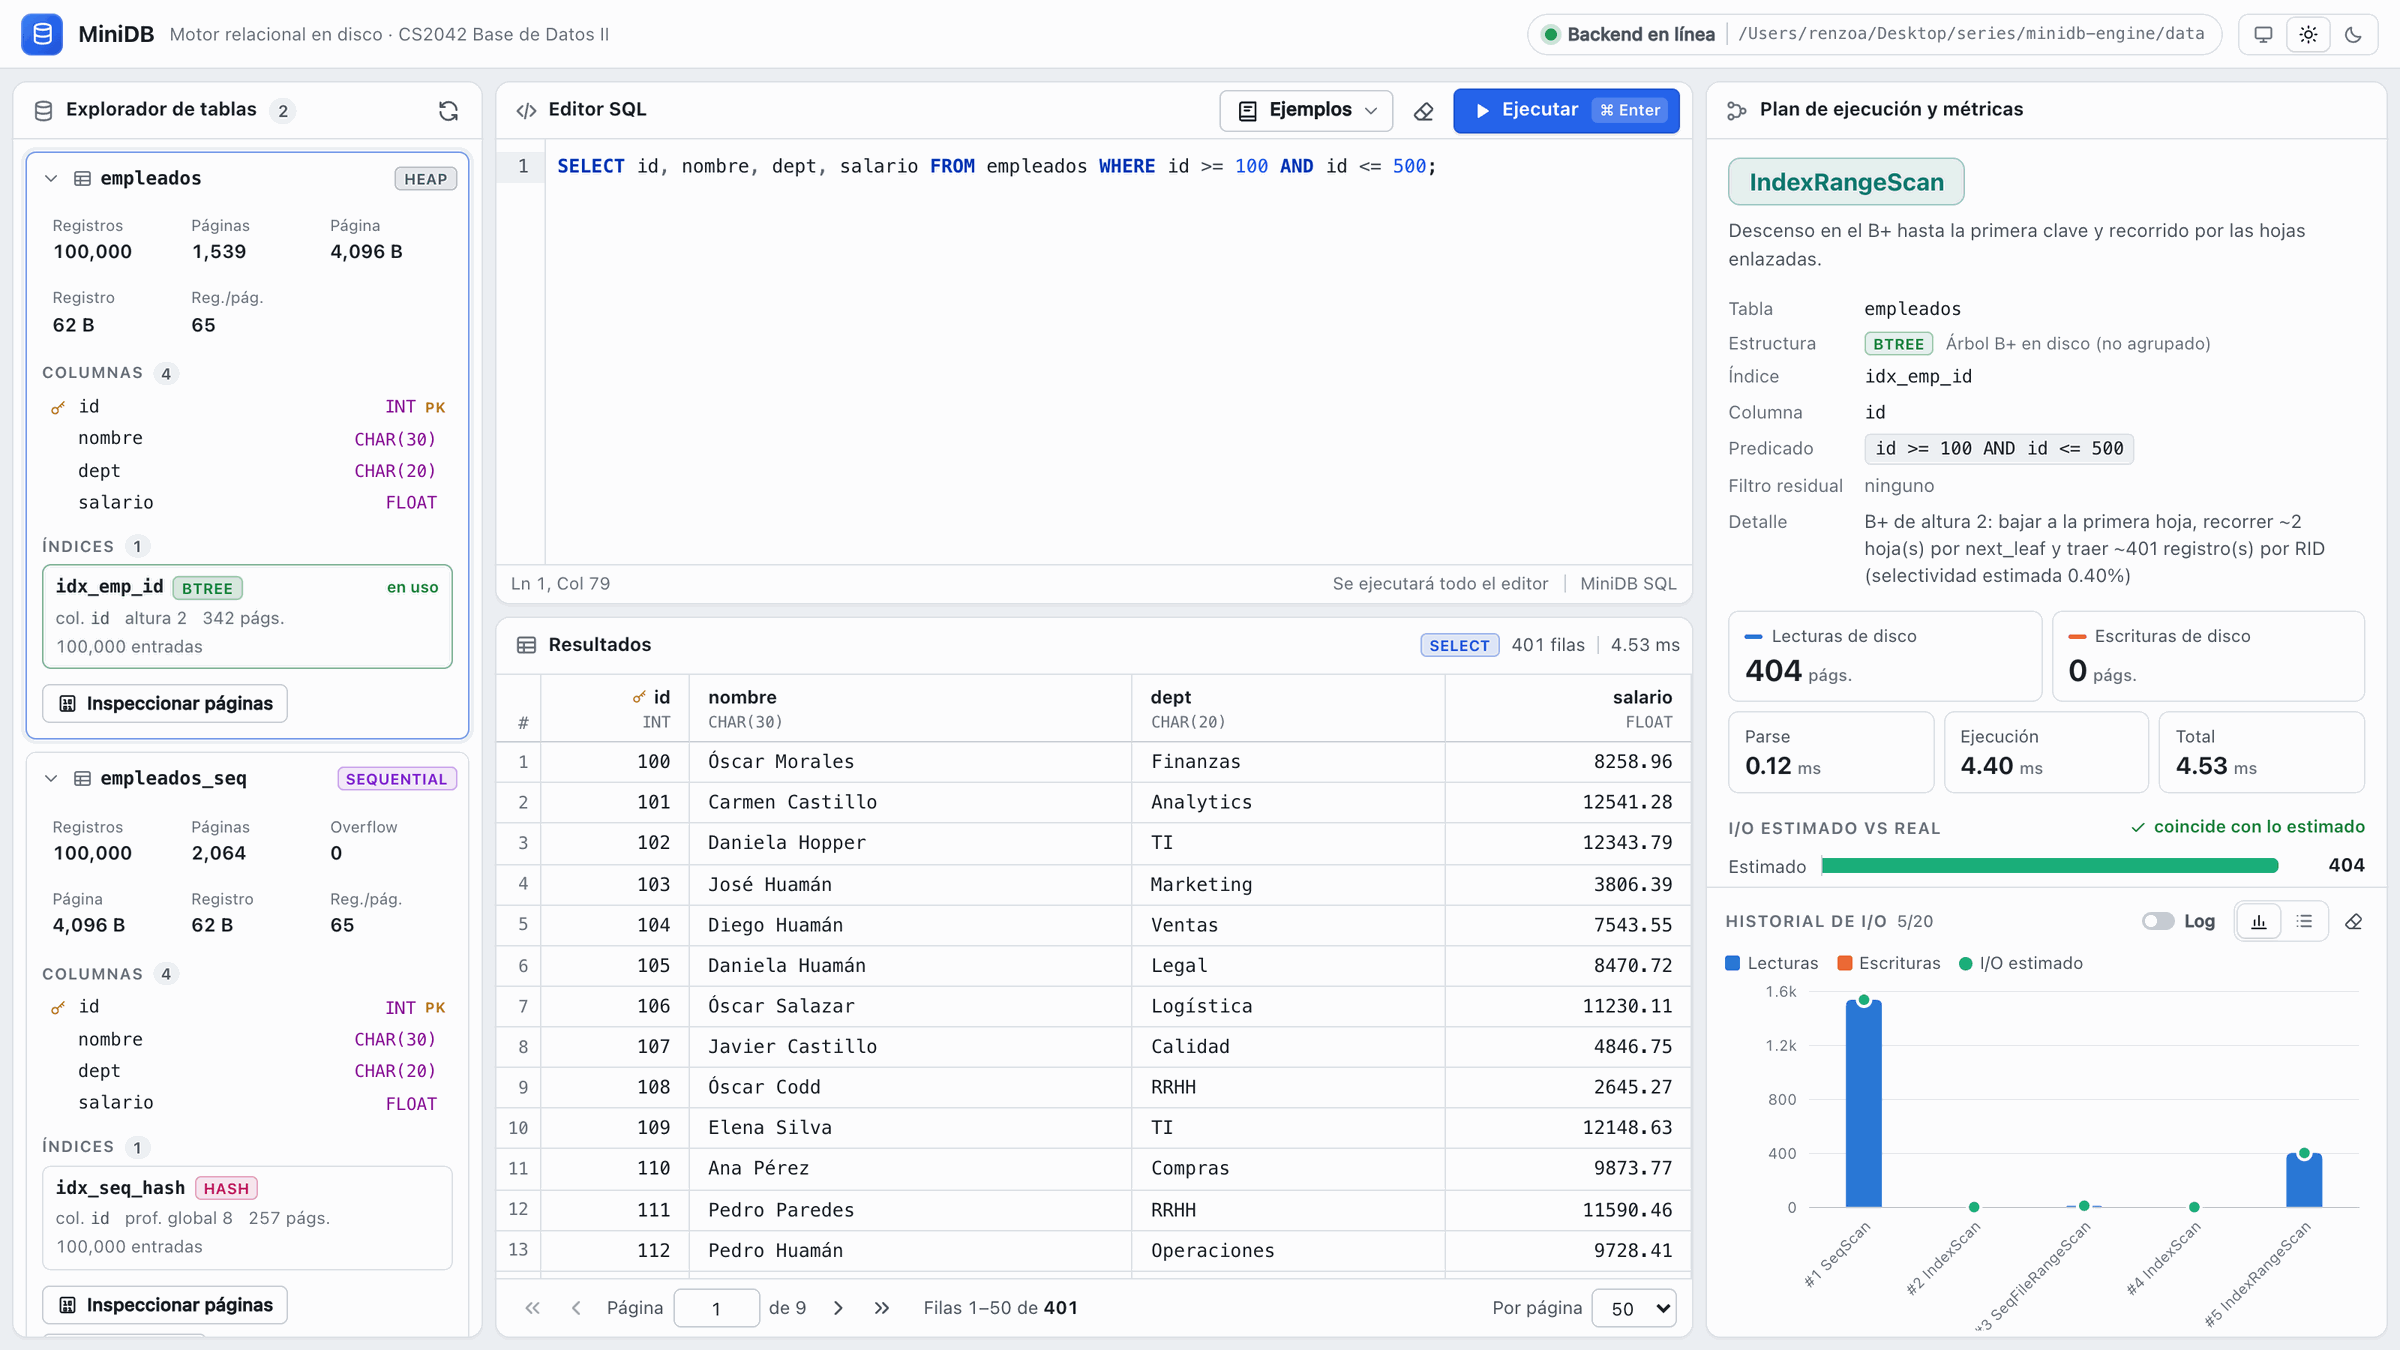
\includegraphics[width=\textwidth]{frontend.png}
\caption{Cliente web con los cuatro paneles: explorador (tabla HEAP con B$^+$ y tabla SEQUENTIAL con
hash), editor SQL, resultados paginados (401 filas) y plan \code{IndexRangeScan} con 404 lecturas, igual
al costo estimado. El historial compara las últimas consultas: \code{SeqScan} (1\,539 lecturas),
\code{IndexScan} (3), \code{SeqFileRangeScan} (13) e \code{IndexRangeScan} (404).}
\label{fig:frontend}
\end{figure}

\begin{figure}[H]
\centering
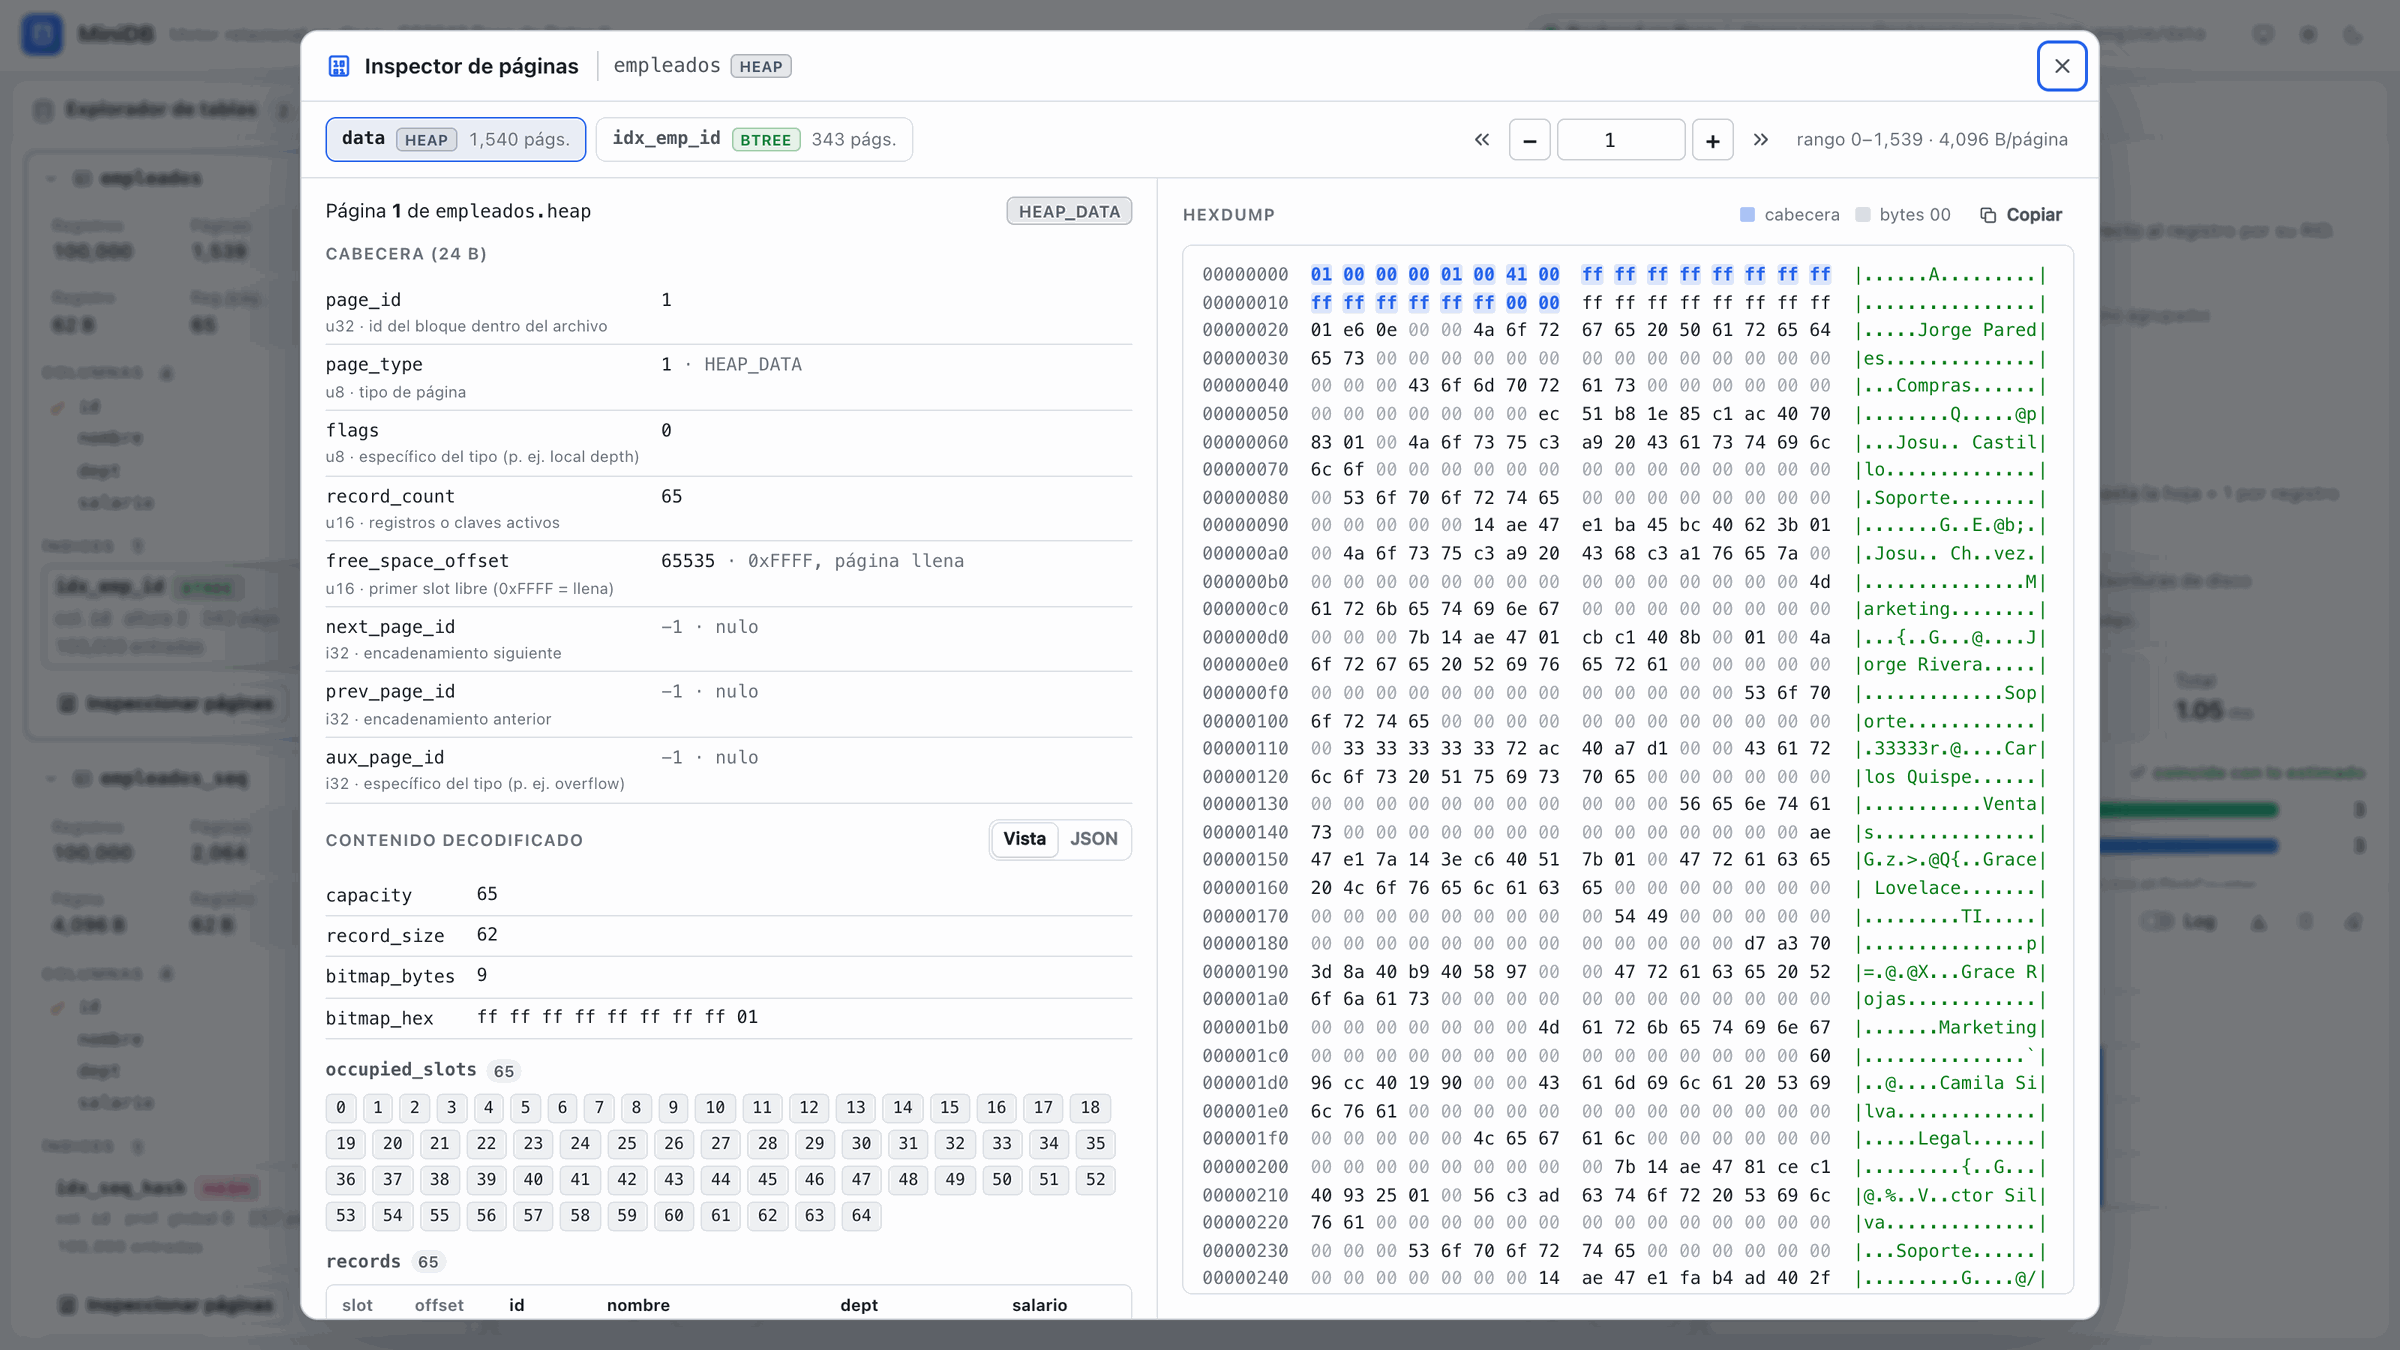
\includegraphics[width=\textwidth]{inspector.png}
\caption{Inspector de páginas (\code{GET /api/tables/\{t\}/pages/\{id\}}): página 1 del Heap. En el
hexdump se ven los 24 bytes del header (\code{page\_id}=1, tipo 1, \code{record\_count} = \code{41 00}
= 65, \code{free\_space\_offset} = \code{ff ff} porque está llena y los punteros en $-1$), el bitmap
(\code{ff}$\times$8 + \code{01} = 65 slots ocupados) y el primer registro: \code{e6 0e 00 00} = id 3814
seguido del nombre en UTF-8.}
\label{fig:inspector}
\end{figure}

%==========================================================================================
\section{Análisis de costos teóricos}

\begin{table}[H]
\centering\small
\begin{tabular}{@{}lllll@{}}
\toprule
Estructura & Inserción & Búsqueda puntual & Rango ($k$ registros) & Eliminación \\
\midrule
Heap (free-list) & 1R + 1W & $P$ (full scan) & $P$ & búsqueda + 1W \\
Sequential & $\lceil\log_2 M\rceil$ + 1W (+ overflow) & $\lceil\log_2 M\rceil$ + ovf. & $\lceil\log_2 M\rceil + \lceil k/r\rceil$ & búsqueda + 1W \\
B$^+$ (índice) & $h$R + 1W (+ split) & $h$ (+1 registro) & $h + \lceil k/f\rceil - 1 + k$ & $h$ + 1W \\
Hash extensible & 2R + 1W (+ split) & 2 (+1 registro) & no soporta & 2R + 1W \\
\bottomrule
\end{tabular}
\caption{Costos en páginas transferidas. $P$: páginas de datos; $M$: páginas principales del
Sequential; $r$: registros por página tras reorganizar ($\lfloor 0.75\,cap\rfloor$); $h$: altura del
B$^+$; $f$: entradas promedio por hoja; $k$: registros que califican.}
\label{tab:costos}
\end{table}

La altura del B$^+$ con $N$ entradas, hojas de capacidad $L$ y fan-out $F$ está acotada por
\[
1+\left\lceil \log_{F}\left\lceil N/L\right\rceil\right\rceil \;\le\; h \;\le\; 1+\left\lceil \log_{\lceil F/2\rceil} \left\lceil N/\lfloor L/2\rfloor\right\rceil \right\rceil,
\]
ya que el split al 50\,\% garantiza nodos al menos a la mitad. El índice es no agrupado, por lo que
un rango paga una lectura aleatoria por registro: frente al full scan ($P$ lecturas) conviene solo si
$k \lesssim P$, es decir, con selectividad menor que $P/N \approx 1/cap$ (1.5\,\% con $B=4096$).
El Sequential, en cambio, está agrupado por la PK: un rango lee páginas contiguas y cuesta
$\approx k/r$ páginas. En el hash el costo de búsqueda no depende de $N$ mientras no haya overflow.

%==========================================================================================
\section{Experimentación}
\label{sec:experimentos}

% Sección de experimentación (se incluye desde informe.tex).
% Las tablas de tablas/*.tex y las figuras de figuras/ se regeneran con:
%   python -m benchmarks.run_all && python -m benchmarks.report_tables

\subsection{Metodología}

Los cuatro experimentos están automatizados en \code{benchmarks/} (\code{python -m benchmarks.run\_all})
y guardan sus resultados en \code{benchmarks/results/} (CSV + PNG). Cada experimento crea archivos nuevos
en una carpeta de trabajo, usa el dataset sintético \code{empleados} generado con semilla fija
(ids únicos 1..$N$ en orden aleatorio, registros de 62 bytes) y mide con contadores independientes
(\code{DiskCounter}) y \code{time.perf\_counter()}, con el recolector de basura desactivado durante las
mediciones. Entorno de la corrida: Python 3.12.13 en macOS-26.3.1-arm64-arm-64bit (10 núcleos), corrida del 2026-09-22 20:28:58
.

Las lecturas y escrituras contadas son \textbf{deterministas} (no dependen de la máquina) y son la métrica
principal. Los tiempos son secundarios: los archivos caben en la caché de páginas del sistema operativo,
de modo que una ``lectura'' cuesta microsegundos y el tiempo refleja sobre todo el costo de CPU de
Python. En un disco real el costo estaría dominado por el número de transferencias.

\paragraph{Reproducibilidad.} Para verificar lo anterior repetimos los experimentos 2, 3 y 4 completos en
una segunda máquina (Windows 11 sobre un AMD64 de 8 núcleos, Python 3.12.1). Todas las columnas de I/O
salen idénticas, incluida la desviación estándar: el full scan lee 1\,539 páginas ($\sigma = 0$), la
búsqueda binaria 11.034 ($\sigma = 0.181$) y el B$^+$ y el hash 3 ($\sigma = 0$); en el Experimento~4
coinciden además el fan-out, la altura, el número de hojas, la I/O de carga y los MB transferidos para
los cuatro tamaños de bloque. Lo único que cambia es el tiempo, de 3 a 10 veces mayor en Windows: la
búsqueda puntual pasa de 0.014--22.7\,ms a 0.051--87.6\,ms según la estructura, un rango del 25\,\% con
el B$^+$ de 109 a 570\,ms, y la carga de los 100\,000 registros del Experimento~4 de 3.7--12.1\,s a
19.9--40.9\,s. Las conclusiones no se mueven: en ambas máquinas el B$^+$ le gana al full scan en tiempo
hasta el 5\,\% de selectividad y lo pierde al 10\,\%.

En el Experimento~1 se mide la \emph{inserción estructural} en todas las organizaciones (sin validar la
unicidad de la PK, porque las claves generadas son únicas por construcción): así se compara lo mismo en
todas, ya que el Heap sin índice no valida y los índices B$^+$/hash se miden por separado. En el motor SQL
la unicidad sí se valida (secciones~\ref{sec:archivos} y~\ref{sec:indices}).

%------------------------------------------------------------------------------------------
\subsection{Experimento 1: costo de inserción masiva}

Se insertan lotes $N\in\{10^3, 10^4, 5\cdot10^4, 10^5, 2.5\cdot10^5, 5\cdot10^5\}$ con $B=4096$. Los
índices B$^+$ y hash son índices únicos sobre \code{id} de un Heap: se reporta el costo total (heap +
índice) y el del índice solo.

\begin{table}[H]
\centering\scriptsize
\begin{tabular}{@{}lrrrrrr@{}}
\toprule
Estructura & $N=1\,000$ & $N=10\,000$ & $N=50\,000$ & $N=100\,000$ & $N=250\,000$ & $N=500\,000$ \\
\midrule
\multicolumn{7}{@{}l}{\emph{Tiempo total (s)}} \\
Heap & 0.01 & 0.10 & 0.43 & 0.94 & 2.46 & 4.72 \\
Sequential sin reorg & 0.01 & 0.12 & 0.63 & 1.31 & 3.22 & 6.52 \\
Sequential con reorg & 0.03 & 0.32 & 1.89 & 4.50 & 12.41 & 24.79 \\
B+ & 0.06 & 0.57 & 4.13 & 7.70 & 22.25 & 42.12 \\
Hash & 0.03 & 0.23 & 1.32 & 2.53 & 5.98 & 12.30 \\
\midrule
\multicolumn{7}{@{}l}{\emph{Escrituras de páginas}} \\
Heap & 1\,001 & 10\,001 & 50\,001 & 100\,001 & 250\,001 & 500\,001 \\
Sequential sin reorg & 1\,016 & 10\,154 & 50\,770 & 101\,539 & 253\,847 & 507\,693 \\
Sequential con reorg & 1\,108 & 10\,918 & 55\,077 & 110\,975 & 273\,965 & 547\,805 \\
B+ & 2\,009 & 20\,090 & 100\,516 & 201\,013 & 502\,889 & 1\,005\,706 \\
Hash & 2\,010 & 20\,069 & 100\,263 & 200\,520 & 502\,059 & 1\,004\,109 \\
\midrule
\multicolumn{7}{@{}l}{\emph{Lecturas de páginas}} \\
Heap & 984 & 9\,846 & 49\,230 & 98\,461 & 246\,153 & 492\,307 \\
Sequential sin reorg & 1\,933 & 19\,933 & 99\,933 & 199\,933 & 499\,933 & 999\,933 \\
Sequential con reorg & 3\,288 & 62\,843 & 429\,335 & 958\,162 & 2\,723\,390 & 5\,946\,007 \\
B+ & 2\,576 & 29\,463 & 148\,987 & 298\,383 & 855\,355 & 1\,851\,665 \\
Hash & 2\,989 & 29\,882 & 149\,364 & 298\,724 & 747\,186 & 1\,494\,366 \\
\midrule
\multicolumn{7}{@{}l}{\emph{I/O por inserción (lecturas + escrituras) / N}} \\
Heap & 1.99 & 1.98 & 1.98 & 1.98 & 1.98 & 1.98 \\
Sequential sin reorg & 2.95 & 3.01 & 3.01 & 3.01 & 3.02 & 3.02 \\
Sequential con reorg & 4.40 & 7.38 & 9.69 & 10.69 & 11.99 & 12.99 \\
B+ & 4.58 & 4.96 & 4.99 & 4.99 & 5.43 & 5.71 \\
Hash & 5.00 & 5.00 & 4.99 & 4.99 & 5.00 & 5.00 \\
\midrule
\multicolumn{7}{@{}l}{\emph{Solo el índice (sin el heap): I/O por inserción}} \\
B+ & 2.60 & 2.97 & 3.01 & 3.01 & 3.45 & 3.73 \\
Hash & 3.01 & 3.01 & 3.01 & 3.01 & 3.01 & 3.01 \\
\bottomrule
\end{tabular}

\caption{Experimento 1: tiempo, escrituras, lecturas e I/O por inserción ($B=4096$).}
\label{tab:exp1}
\end{table}

\begin{figure}[H]
\centering
\begin{subfigure}{0.49\textwidth}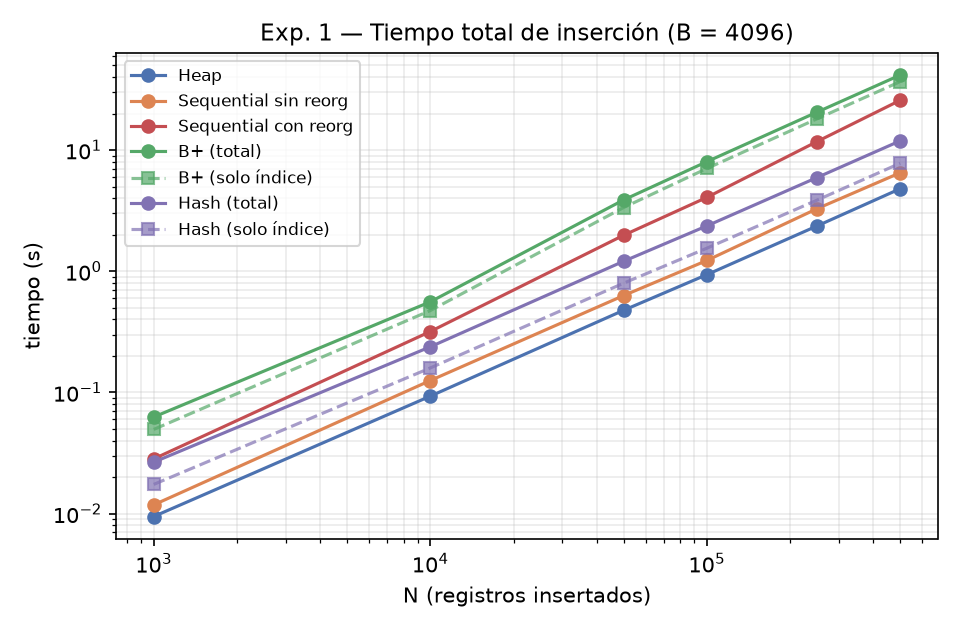
\includegraphics[width=\textwidth]{exp1_time.png}\caption{Tiempo total.}\end{subfigure}
\begin{subfigure}{0.49\textwidth}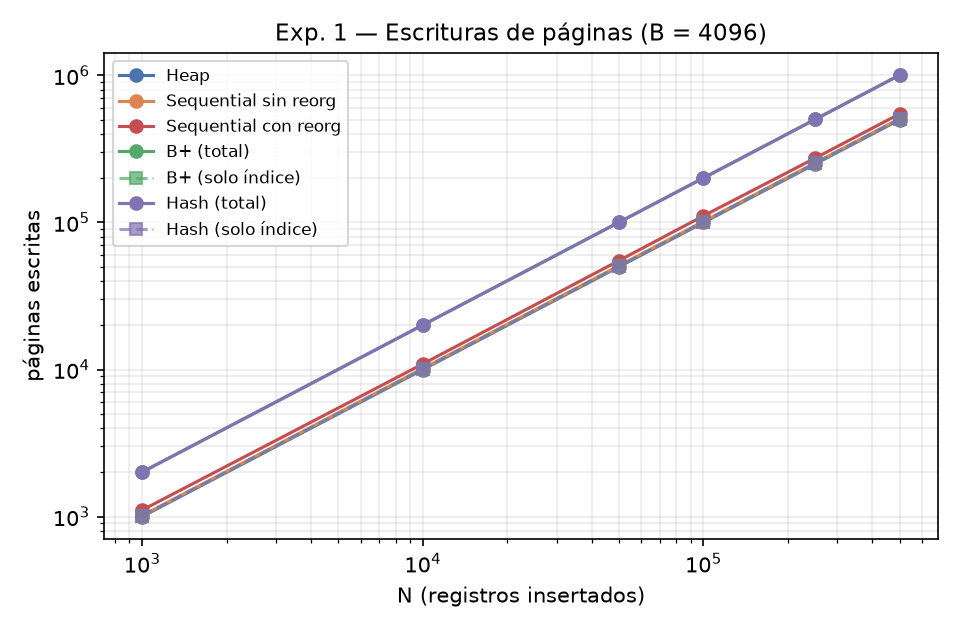
\includegraphics[width=\textwidth]{exp1_writes.png}\caption{Escrituras.}\end{subfigure}
\caption{Experimento 1 en escala log-log: todas las curvas son lineales en $N$ (pendiente 1), es decir,
costo por inserción aproximadamente constante.}
\label{fig:exp1a}
\end{figure}

\begin{figure}[H]
\centering
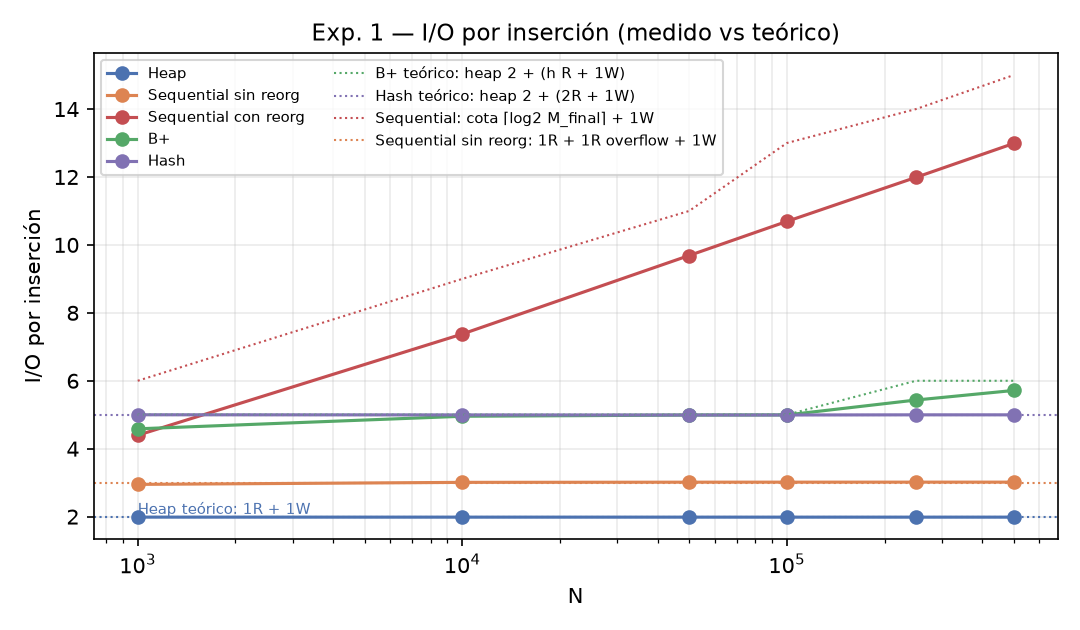
\includegraphics[width=0.78\textwidth]{exp1_io_per_insert.png}
\caption{I/O por inserción medido frente al costo teórico.}
\label{fig:exp1b}
\end{figure}

\paragraph{Análisis.}
\begin{itemize}
\item \textbf{Heap}: 1.98 I/O por inserción para todo $N$, exactamente el costo teórico de 1R + 1W
  (el 0.02 que falta son las inserciones que abren una página nueva, que cuestan solo 1W: una de cada 65).
  Es la inserción más barata y la más rápida ($\approx 4.8$\,s para 500\,000 registros).
\item \textbf{Sequential sin reorganización}: $\approx 3$ I/O por inserción (1R de la página principal,
  1R + 1W de la cabeza de su overflow). La inserción es barata, pero el archivo degenera: con 500\,000
  registros queda 1 página principal y 7\,692 de overflow, y una búsqueda puntual posterior cuesta en
  promedio 4\,026 lecturas (tabla~\ref{tab:exp1seq}, figura~\ref{fig:exp1c}); es decir, sin reorganizar el
  Sequential se comporta como un Heap con peor inserción.
\item \textbf{Sequential con reorganización}: el costo por inserción crece como $\log_2 M$ (4.4 I/O con
  1\,000 registros, 13.0 con 500\,000): cada inserción paga la búsqueda binaria de su página. Las
  reorganizaciones (35 en total para 500\,000 registros) suman solo $\approx 0.1$ escrituras por
  inserción, porque el archivo crece geométricamente entre una y otra (con fill factor 0.75 cada página
  admite $\approx 35$\,\% más registros antes de desbordar: pasa de 48 a 65). A cambio, al terminar la carga la búsqueda
  cuesta $\lceil\log_2 M\rceil\approx 13$ lecturas.
\item \textbf{B$^+$}: el índice solo cuesta $h$R + 1W: 3.0 I/O por inserción mientras $h=2$ y 3.7 con
  500\,000 claves, cuando la altura pasa a 3 (tabla~\ref{tab:exp1forma}); los splits agregan poco
  (una hoja se divide cada $\approx 290$ inserciones). Es la estructura más lenta en tiempo porque cada
  inserción decodifica y reescribe nodos de hasta 508 claves.
\item \textbf{Hash}: 3.0 I/O por inserción del índice para todo $N$ (2R + 1W), independiente de $N$; la
  profundidad global crece de 2 a 11 y el directorio ocupa 1 a 3 páginas. Los splits y las
  duplicaciones del directorio son poco frecuentes, y \code{crc32} reparte las claves de forma tan
  uniforme que los buckets quedan casi llenos (96\,\% de ocupación con 100\,000 claves).
\end{itemize}

\begin{table}[H]
\centering\small
\begin{tabular}{@{}lrrrrrr@{}}
\toprule
$N$ & \multicolumn{3}{c}{Sequential sin reorg} & \multicolumn{3}{c}{Sequential con reorg} \\
\cmidrule(lr){2-4}\cmidrule(l){5-7}
 & $M$ & overflow & búsqueda & $M$ & overflow (reorgs) & búsqueda \\
\midrule
1\,000 & 1 & 15 & 9.5 & 19 & 0 (8) & 4.4 \\
10\,000 & 1 & 153 & 79.9 & 168 & 7 (17) & 7.4 \\
50\,000 & 1 & 769 & 394.3 & 957 & 0 (25) & 9.9 \\
100\,000 & 1 & 1\,538 & 742.2 & 2\,064 & 0 (28) & 11.0 \\
250\,000 & 1 & 3\,846 & 1\,742.6 & 4\,509 & 8 (32) & 12.2 \\
500\,000 & 1 & 7\,692 & 4\,026.3 & 9\,045 & 22 (35) & 13.1 \\
\bottomrule
\end{tabular}

\caption{Sequential File tras la carga: páginas principales ($M$), páginas de overflow y lecturas
promedio de una búsqueda puntual posterior (100 claves aleatorias).}
\label{tab:exp1seq}
\end{table}

\begin{table}[H]
\centering\footnotesize\setlength{\tabcolsep}{4pt}
\begin{tabular}{@{}lrrrrrr@{}}
\toprule
Estructura & $N=1\,000$ & $N=10\,000$ & $N=50\,000$ & $N=100\,000$ & $N=250\,000$ & $N=500\,000$ \\
\midrule
B$^+$: altura $h$ & 2 & 2 & 2 & 2 & 3 & 3 \\
Hash: profundidad global & 2 & 5 & 7 & 8 & 10 & 11 \\
\bottomrule
\end{tabular}

\caption{Forma final de los índices en el Experimento 1.}
\label{tab:exp1forma}
\end{table}

\begin{figure}[H]
\centering
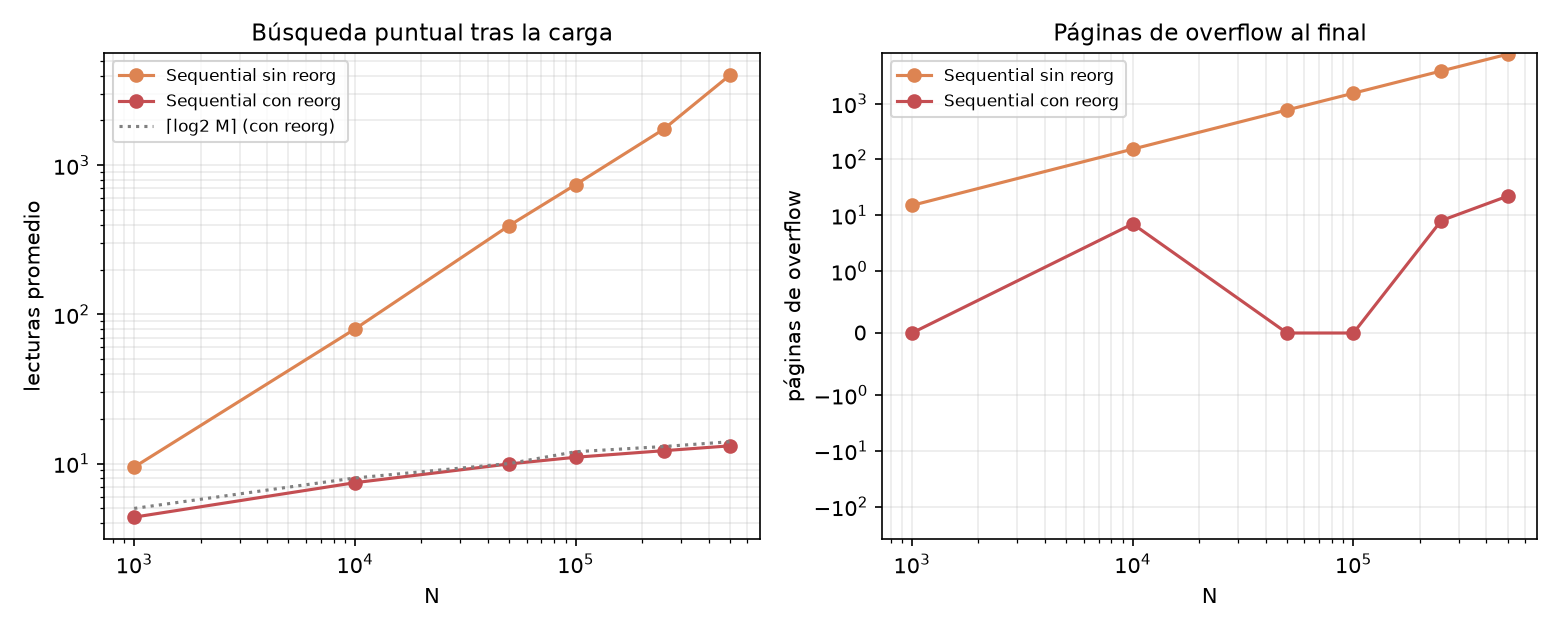
\includegraphics[width=0.92\textwidth]{exp1_sequential_reorg.png}
\caption{Lo que compra la reorganización: sin ella la búsqueda posterior es lineal en $N$ (la cadena de
overflow crece sin límite); con ella se mantiene en $\lceil\log_2 M\rceil$.}
\label{fig:exp1c}
\end{figure}

%------------------------------------------------------------------------------------------
\subsection{Experimento 2: búsquedas puntuales de igualdad}

Con $N=100\,000$ registros ($B=4096$) se ejecutan 1\,000 búsquedas de claves aleatorias existentes en
cada estructura. Las lecturas incluyen traer el registro por RID en los índices.

\begin{table}[H]
\centering\footnotesize\setlength{\tabcolsep}{4pt}
\begin{tabular}{@{}lrrrrrl@{}}
\toprule
Método & lecturas (media) & $\sigma$ & teórico & ms (media) & $\sigma$ (ms) & parámetros \\
\midrule
Full Scan (Heap) & 1\,539.00 & 0.00 & 1\,539 & 22.504 & 4.136 & P = 1539 páginas \\
Búsqueda binaria (Sequential) & 11.03 & 0.18 & 11.03 & 0.093 & 0.206 & M = 2084 páginas principales \\
B$^+$ (IndexScan) & 3.00 & 0.00 & 3 & 0.039 & 0.016 & h = 2 \\
Hash (IndexScan) & 3.00 & 0.00 & 3 & 0.013 & 0.004 & global depth = 8 \\
\bottomrule
\end{tabular}

\caption{Experimento 2: 1\,000 búsquedas de igualdad sobre 100\,000 registros.}
\label{tab:exp2}
\end{table}

\begin{figure}[H]
\centering
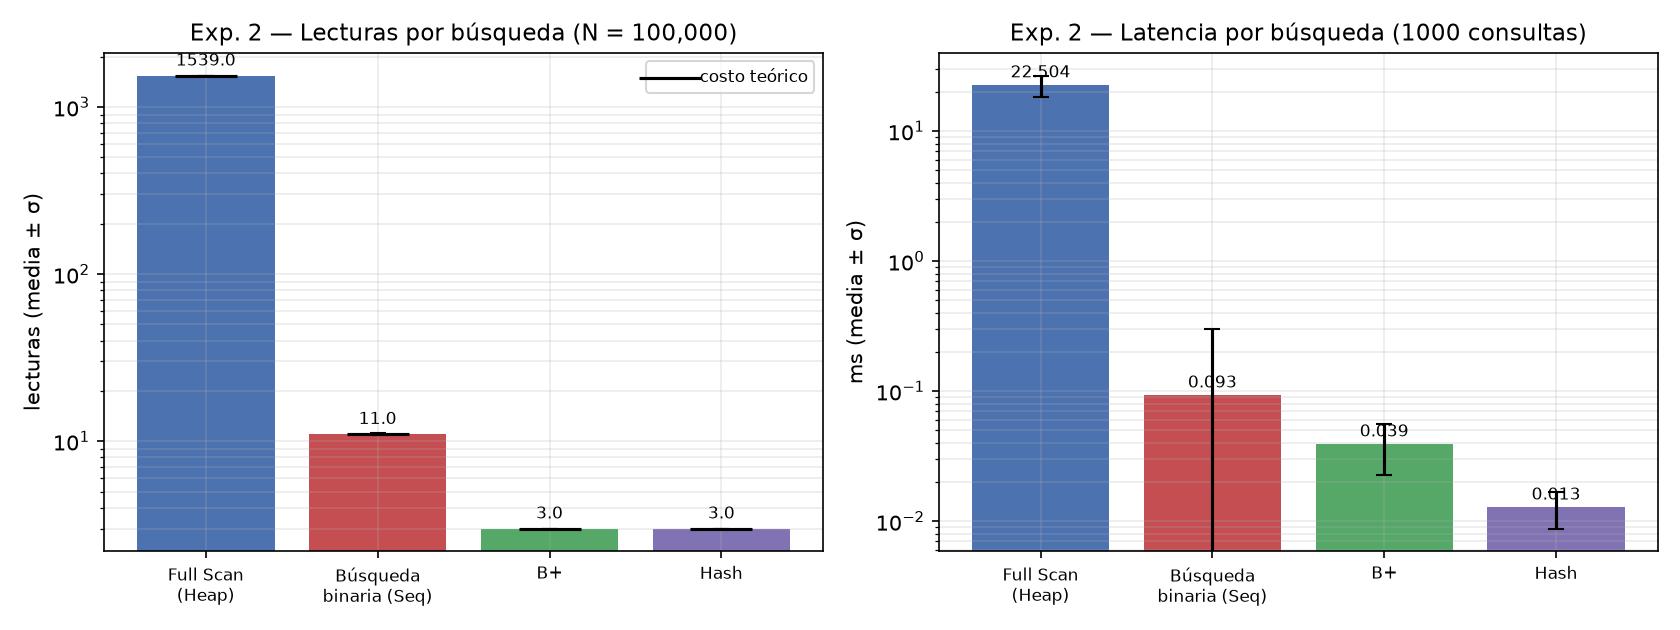
\includegraphics[width=\textwidth]{exp2_equality.png}
\caption{Experimento 2 (escala logarítmica). La raya negra marca el costo teórico.}
\label{fig:exp2}
\end{figure}

\paragraph{Análisis.} Los cuatro métodos coinciden con la teoría:
el \textbf{full scan} lee siempre las $P=1\,539$ páginas ($\sigma=0$), la \textbf{búsqueda binaria} sobre
$M=2\,084$ páginas principales hace en promedio $\log_2 M = 11.03$ sondeos ($\lfloor\log_2 M\rfloor$ o
$\lceil\log_2 M\rceil$ según la clave, de ahí $\sigma=0.18$), el \textbf{B$^+$} de altura $h=2$ cuesta
exactamente $h+1=3$ lecturas y el \textbf{hash} exactamente 3 (directorio + bucket + registro, sin
overflow). El índice reduce el costo en un factor de $\approx 500$ frente al full scan. En tiempo, B$^+$
y hash hacen las mismas 3 lecturas pero el hash es casi 3 veces más rápido: busca la clave en el bucket con
una búsqueda de bytes en C, mientras que el B$^+$ decodifica dos nodos completos con \code{struct}. La
búsqueda binaria es $\approx 250$ veces más rápida que el full scan a pesar de no usar índice.

%------------------------------------------------------------------------------------------
\subsection{Experimento 3: búsquedas por rango con selectividad variable}
\label{sec:exp3}

Con $N=100\,000$ ($B=4096$) se consultan rangos \code{id BETWEEN a AND a+k-1} que devuelven el 0.1\,\%,
1\,\%, 5\,\%, 10\,\% y 25\,\% de la tabla (10 rangos aleatorios por selectividad).

\begin{table}[H]
\centering\scriptsize
\begin{tabular}{@{}lrrrrrrrrrr@{}}
\toprule
 & & \multicolumn{3}{c}{B$^+$} & \multicolumn{3}{c}{Sequential} & \multicolumn{3}{c}{Full Scan (Heap)} \\
\cmidrule(lr){3-5}\cmidrule(lr){6-8}\cmidrule(lr){9-11}
Selectividad & $k$ & lecturas & teórico & ms & lecturas & teórico & ms & lecturas & teórico & ms \\
\midrule
0.1\,\% & 100 & 102.3 & 102.0 & 1.64 & 13.2 & 13.1 & 0.25 & 1\,539.0 & 1\,539.0 & 24.14 \\
1\,\% & 1\,000 & 1\,005.5 & 1\,005.0 & 4.05 & 31.8 & 31.9 & 1.55 & 1\,539.0 & 1\,539.0 & 25.05 \\
5\,\% & 5\,000 & 5\,018.8 & 5\,019.0 & 20.60 & 115.2 & 115.2 & 7.47 & 1\,539.0 & 1\,539.0 & 29.76 \\
10\,\% & 10\,000 & 10\,037.2 & 10\,036.0 & 42.06 & 219.5 & 219.4 & 17.34 & 1\,539.0 & 1\,539.0 & 35.86 \\
25\,\% & 25\,000 & 25\,087.8 & 25\,087.0 & 105.57 & 531.7 & 531.9 & 36.17 & 1\,539.0 & 1\,539.0 & 51.48 \\
\bottomrule
\end{tabular}

\caption{Experimento 3: lecturas medidas (media de 10 rangos), costo teórico y tiempo en ms.
Teórico: B$^+$ $= h + \lceil k/f\rceil - 1 + k$; Sequential $= \log_2 M + k/r$ con $r=48$; full scan $=P$.}
\label{tab:exp3}
\end{table}

\begin{figure}[H]
\centering
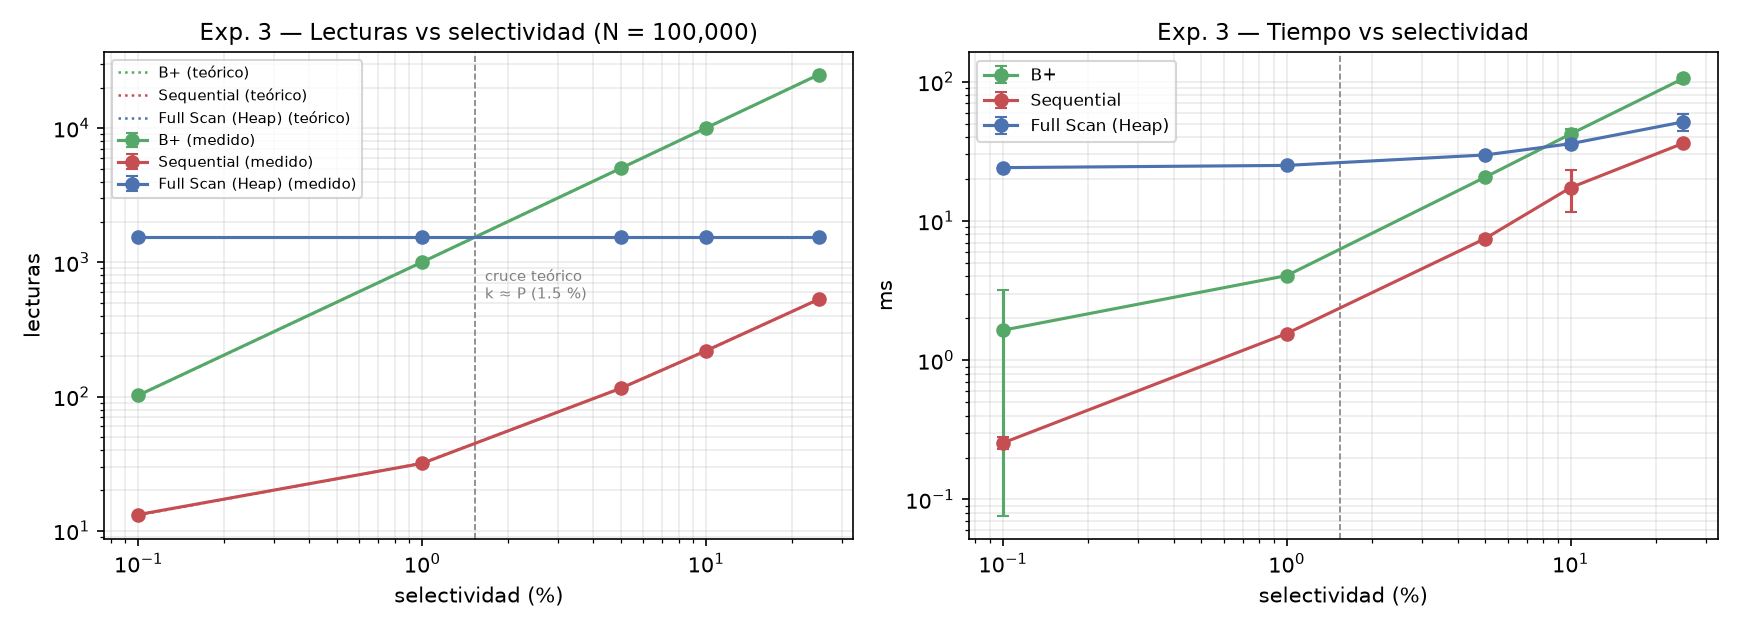
\includegraphics[width=\textwidth]{exp3_range.png}
\caption{Experimento 3: lecturas y tiempo frente a la selectividad (log-log). La línea vertical marca
el cruce teórico entre el B$^+$ no agrupado y el full scan ($k\approx P$).}
\label{fig:exp3}
\end{figure}

\paragraph{Análisis.}
\begin{itemize}
\item \textbf{B$^+$ (no agrupado)}: cuesta $\approx k$ lecturas (una por registro, porque cada RID apunta
  a una página distinta del Heap) más $h$ y las hojas recorridas (1 hoja cada $\approx 290$ entradas).
  Supera al full scan cuando $k > P$, es decir, con selectividad mayor a $P/N = 1.5$\,\%: con 25\,\%
  hace 25\,088 lecturas, 16 veces más que el full scan. Este es el cruce que justifica que un
  optimizador basado en costos (modo \code{cost} de nuestro planner) elija el full scan para rangos
  amplios.
\item \textbf{Sequential (agrupado)}: la búsqueda binaria ubica la primera página ($\log_2 M\approx 11$
  lecturas) y luego lee páginas contiguas con 48 registros cada una: $k/48$ páginas. Es el mejor método en
  todas las selectividades (532 lecturas para el 25\,\%, un tercio del full scan) y el costo medido
  coincide con la fórmula a la décima.
\item \textbf{Full scan}: $P=1\,539$ lecturas constantes; solo crece el tiempo de CPU (filtrar y
  decodificar más filas).
\item \textbf{Tiempo vs I/O}: en tiempo el B$^+$ le gana al full scan hasta $\approx 5$\,\% aunque ya lea
  3 veces más páginas, porque sus lecturas aleatorias caen en la caché del sistema operativo y cuestan
  poco; en un disco real, donde una lectura aleatoria cuesta de 0.1\,ms (SSD) a varios ms (HDD), el cruce
  se acerca al que predice el conteo de I/O (1.5\,\%).
\end{itemize}

%------------------------------------------------------------------------------------------
\subsection{Experimento 4: sensibilidad al tamaño de bloque}

Para $B\in\{1024, 2048, 4096, 8192\}$ se insertan 100\,000 registros en un Heap con un B$^+$ único sobre
\code{id} y luego se hacen 1\,000 búsquedas puntuales. Como referencia se reporta también el Sequential
(reorganizado) y el hash con el mismo $B$.

\begin{table}[H]
\centering\small
\begin{tabular}{@{}lrrrr@{}}
\toprule
$B$ (bytes) & 1\,024 & 2\,048 & 4\,096 & 8\,192 \\
\midrule
registros por página del heap & 16 & 32 & 65 & 131 \\
páginas del heap ($P$) & 6\,250 & 3\,125 & 1\,539 & 764 \\
entradas por hoja ($L$) & 100 & 202 & 407 & 816 \\
fan-out del interno ($m+1$) & 125 & 253 & 509 & 1\,021 \\
altura $h$ medida & 3 & 3 & 2 & 2 \\
altura teórica [mín, máx] & [3, 3] & [3, 3] & [2, 3] & [2, 2] \\
hojas / internos & 1\,422 / 17 & 714 / 5 & 341 / 1 & 161 / 1 \\
I/O de inserción (heap + B$^+$) & 591\,248 & 563\,984 & 499\,396 & 499\,046 \\
\quad de los cuales en el B$^+$ & 397\,497 & 367\,108 & 300\,934 & 299\,809 \\
lecturas por búsqueda ($h+1$) & 4.00 & 4.00 & 3.00 & 3.00 \\
I/O total (inserción + 1000 búsquedas) & 595\,248 & 567\,984 & 502\,396 & 502\,046 \\
MB transferidos (I/O $\times B$) & 581.3 & 1\,109.3 & 1\,962.5 & 3\,922.2 \\
tiempo de inserción (s) & 3.70 & 5.44 & 7.53 & 12.08 \\
Sequential: $M$ / lecturas por búsqueda & 8\,334 / 13.04 & 4\,167 / 12.03 & 2\,084 / 11.04 & 1\,021 / 10.00 \\
Hash: profundidad global / buckets & 10 / 1\,024 & 9 / 512 & 8 / 256 & 7 / 128 \\
\bottomrule
\end{tabular}

\caption{Experimento 4: efecto del tamaño de página ($N=100\,000$). La altura teórica es el intervalo
entre nodos llenos y nodos al 50\,\%.}
\label{tab:exp4}
\end{table}

\begin{figure}[H]
\centering
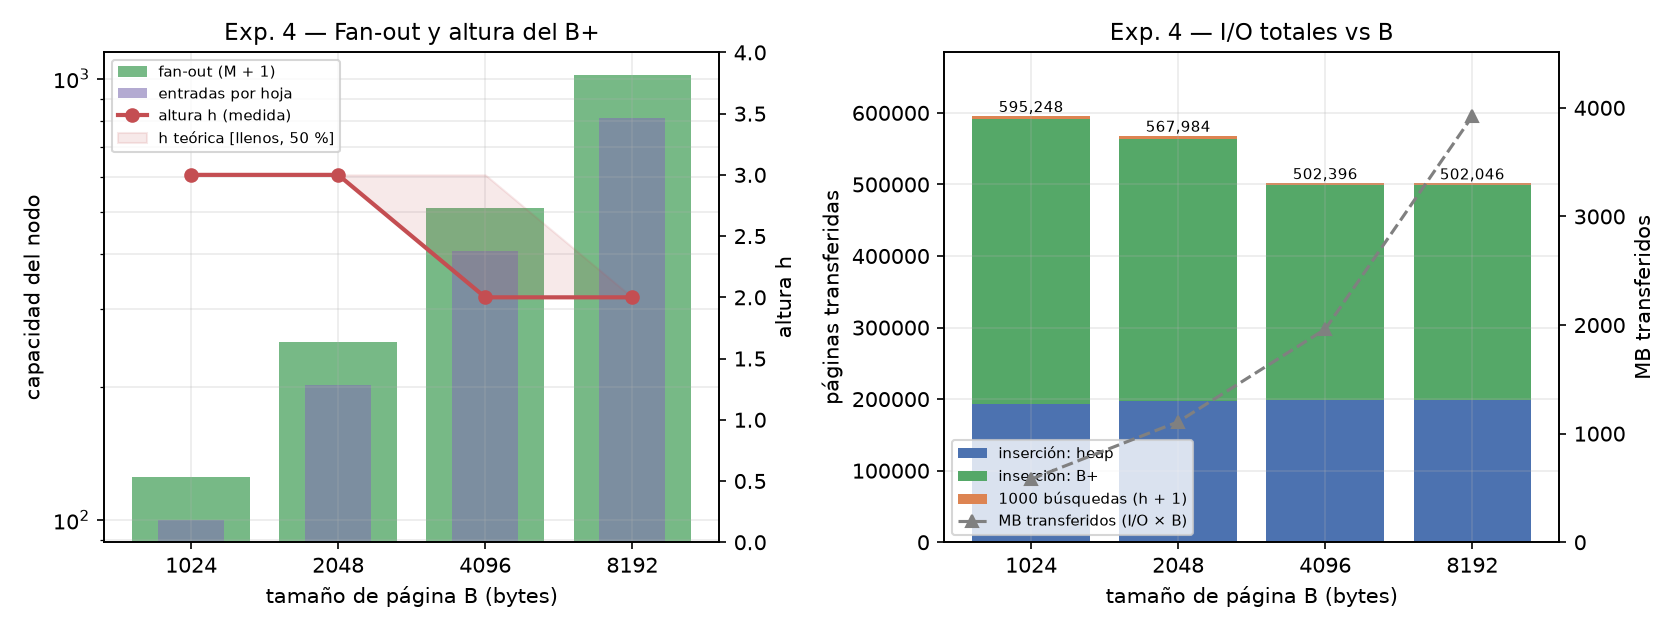
\includegraphics[width=\textwidth]{exp4_block_size.png}
\caption{Experimento 4: fan-out y altura del B$^+$ (izq.) e I/O totales y bytes transferidos (der.).}
\label{fig:exp4}
\end{figure}

\begin{figure}[H]
\centering
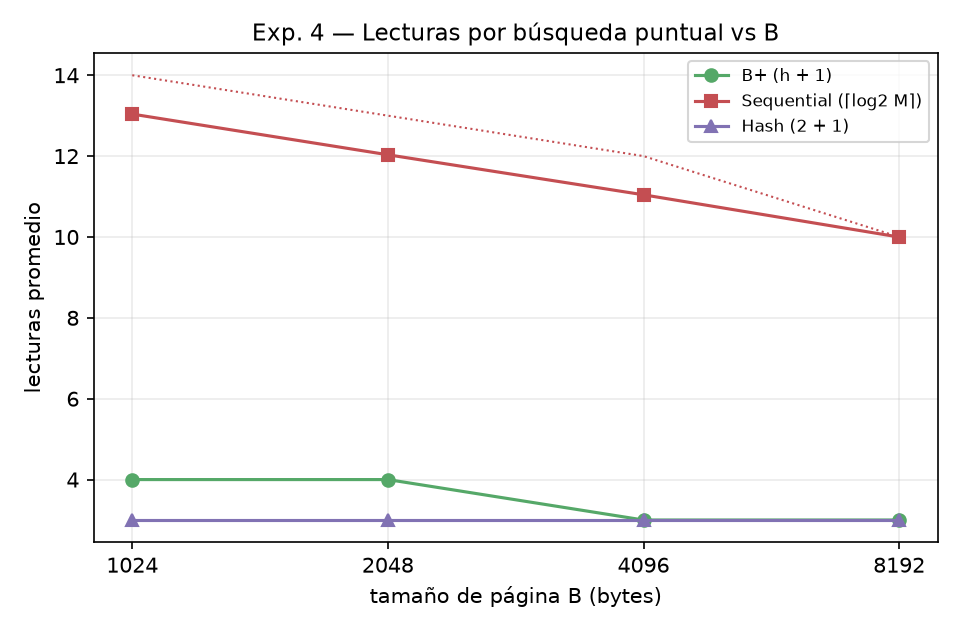
\includegraphics[width=0.62\textwidth]{exp4_search_reads.png}
\caption{Lecturas por búsqueda puntual según $B$: B$^+$ ($h+1$), Sequential ($\log_2 M$) y hash (3).}
\label{fig:exp4b}
\end{figure}

\paragraph{Análisis.} El fan-out crece linealmente con $B$ (125, 253, 509 y 1\,021) y la altura baja de
3 a 2 al pasar de 2\,048 a 4\,096 bytes, siempre dentro del intervalo teórico. Como cada búsqueda cuesta
$h+1$, pasa de 4 a 3 lecturas, y como cada inserción cuesta $h$R + 1W en el índice, las I/O de inserción
del B$^+$ bajan de 397\,497 a 299\,809 (las del Heap, 2 por registro, no dependen de $B$). El total de
I/O baja un 16\,\% de $B=1024$ a $B=8192$, pero el volumen transferido (I/O $\times B$) crece casi
linealmente: de 581\,MB a 3\,922\,MB. Duplicar $B$ más allá de 4\,096 no reduce la altura para
100\,000 claves (la raíz ya cabe en una página) y solo encarece cada transferencia: páginas de 4\,KB,
el tamaño de página del sistema operativo, son el mejor compromiso para este volumen. El Sequential
muestra el mismo efecto ($\log_2 M$ baja de 13 a 10 lecturas) y el hash mantiene 3 lecturas con
cualquier $B$, con una profundidad global que baja de 10 a 7 porque los buckets son más grandes.


%==========================================================================================
\section{Pruebas}

La suite de \code{pytest} (\code{tests/}, un archivo por módulo) cubre: round-trip de header,
página, registro, RID y metadatos; \textbf{exactitud del contador} (inserción en Heap con página
libre = 1R + 1W, búsqueda en B$^+$ = $h$ lecturas, full scan = $P$ lecturas, hash = 2 lecturas,
búsqueda binaria $\le\lceil\log_2 M\rceil + 1$); invariantes del B$^+$ tras 20\,000 inserciones
aleatorias (claves ordenadas en cada nodo, cotas de los separadores, hojas enlazadas en ambos
sentidos, todas a la misma profundidad, nodos al menos al 50\,\% y altura entre las cotas de
$\log_M N$); hash con duplicados, profundidad máxima y splits del directorio en varias páginas;
\code{reorganize} (conserva registros, vacía el overflow, respeta el fill factor y usa ordenamiento
externo con cadenas largas); persistencia (cerrar, reabrir y obtener los mismos resultados); parser
(casos válidos y errores con posición); planner y ejecutor de punta a punta; y la API REST. Además,
pruebas aleatorias \emph{diferenciales} ejecutan miles de inserciones, borrados y búsquedas sobre
cada estructura (y por SQL, con índices B$^+$ y hash sobre una tabla Sequential) y comparan cada
resultado con un modelo en memoria, con páginas de 512 bytes para forzar splits, overflow,
reorganizaciones y cierres/reaperturas. En total son 133 pruebas que corren en $\approx 12$\,s.

%==========================================================================================
\section{Conclusiones}

\begin{itemize}
\item Contar las páginas transferidas (y no solo el tiempo) permite verificar la teoría con exactitud:
  los costos medidos coinciden con las fórmulas de la tabla~\ref{tab:costos} en todos los
  experimentos.
\item El Heap tiene la inserción más barata (2 I/O) pero toda búsqueda sin índice cuesta $P$.
\item El Sequential File ofrece búsquedas en $\lceil\log_2 M\rceil$ y los rangos más baratos por estar
  agrupado, a cambio de reorganizar periódicamente: sin reorganización la inserción es barata pero
  el archivo degenera en una cadena de overflow y la búsqueda se vuelve lineal.
\item El B$^+$ da búsquedas en $h+1$ con $h$ muy baja (2--3 para 100\,000 claves) y soporta rangos,
  pero como índice no agrupado pierde frente al full scan cuando la selectividad supera
  $\approx P/N$; ahí el modo \code{cost} del planificador elige el full scan.
\item El hash extensible logra búsquedas en 3 lecturas independientes de $N$, sin soportar rangos.
\item Páginas más grandes aumentan el fan-out y reducen la altura y el número de I/O, pero cada I/O
  transfiere más bytes: el volumen transferido crece casi linealmente con $B$.
\end{itemize}

\paragraph{Trabajo futuro.} Buffer pool con política LRU (desactivable para medir), fusión y
redistribución en el B$^+$, recorrido de índice ordenado por página (\emph{bitmap heap scan}),
transacciones con WAL y, para el Entregable~2, los módulos espacial (R-Tree), textual (SPIMI/BM25) y
vectorial (IVF/HNSW).

\begin{thebibliography}{9}
\bibitem{ramakrishnan} R. Ramakrishnan y J. Gehrke. \emph{Database Management Systems}, 3.\textsuperscript{a} ed. McGraw-Hill, 2003.
\bibitem{garcia} H. Garcia-Molina, J. D. Ullman y J. Widom. \emph{Database Systems: The Complete Book}, 2.\textsuperscript{a} ed. Pearson, 2008.
\bibitem{silberschatz} A. Silberschatz, H. F. Korth y S. Sudarshan. \emph{Database System Concepts}, 7.\textsuperscript{a} ed. McGraw-Hill, 2019.
\bibitem{fagin} R. Fagin, J. Nievergelt, N. Pippenger y H. R. Strong. Extendible hashing --- a fast access method for dynamic files. \emph{ACM TODS}, 4(3):315--344, 1979.
\bibitem{comer} D. Comer. The ubiquitous B-tree. \emph{ACM Computing Surveys}, 11(2):121--137, 1979.
\bibitem{selinger} P. G. Selinger et al. Access path selection in a relational database management system. \emph{SIGMOD}, 1979.
\end{thebibliography}

\end{document}
